Als glatte Mannigfaltigkeit sei im Weiteren stets ein zweitabz\"ahlbarer Haus\-dorff-Raum bezeichnet, der sich lokal in den \({\mathbb{K}\in\{\mathbb{R}^{n+1},\mathbb{R}^n\times\mathbb{R}_{\geq0},\mathbb{R}_{\geq0}^{n+1}\}}\) einbetten lasse und mit einer glatten Struktur versehen sei. Im ersten Fall handelt es sich um eine gew\"ohnliche glatte Mannigfaltigkeit, im zweiten um eine glatte Mannigfaltigkeit mit Rand und im dritten um eine glatte Mannigfaltigkeit mit Ecken. Insbesondere sind Mannigfaltigkeiten mit Ecken nicht unbedingt Mannigfaltigkeiten mit Rand. \textbf{Alle Mannigfaltigkeiten seien im Folgenden glatte, kompakte Mannigfaltigkeiten mit (m\"oglicherweise leerem) Rand}. Mannigfaltigkeiten mit leerem Rand hei\ss en geschlossen. 

\section{Kobordismen}\label{sec:cobordism}
    \begin{definition}[Kobordismus]\label{def:cobordism}
        Seien \({\mathcal{M}^n}\) und \({\mathcal{N}^n}\) geschlossene Mannigfaltigkeiten, so hei\ss e eine Mannigfaltigkeit \({\mathcal{W}^{n+1}}\) mit einer Zerlegung \({\partial\mathcal{W}\cong\mathcal{M}\sqcup\mathcal{N}}\) ein Kobordismus von \({\mathcal{M}}\) zu \({\mathcal{N}}\).
    \end{definition}
    Es werde gelegentlich auch die Notation \({\partial_-\mathcal{W}:=\mathcal{M}}\) und \({\partial_+\mathcal{W}:=\mathcal{N}}\) genutzt.

    \begin{definition}[Diffeomorphie zweier Kobordismen]\label{def:diffeomorphic_cobordism}
        Zwei Kobordismen \({\mathfrak{W}=\left(\mathcal{W},\mathcal{M},\mathcal{N}\right)}\) und \({\mathfrak{W}^{\prime}=\left(\mathcal{W}^{\prime},\mathcal{M},\mathcal{N}^{\prime}\right)}\) hei\ss en diffeomorph relativ zu \({\mathcal{M}}\) (im Folgenden einfach diffeomorph), falls das Diagramm 
        \begin{center}
            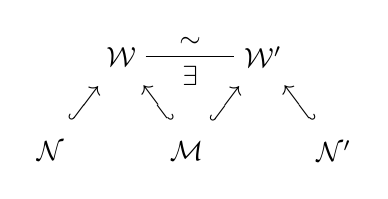
\begin{tikzpicture}[scale = 1.2]
                \draw 
                    node (A) at (-1.5, -1) {\({\mathcal{N}}\)}
                    node (B) at (-0.75, 0) {\({\mathcal{W}}\)}
                    node (C) at (0.75, 0) {\({\mathcal{W}^{\prime}}\)}
                    node (D) at (1.5, -1) {\({\mathcal{N}^{\prime}}\)}
                    node (E) at (0, -1) {\({\hspace{-4pt}\mathcal{M}}\)}
                    (B) -- node [above] {\({\sim}\)} node [below] {\({\exists}\)} (C);
                \path
                    (A) -- node [sloped] {\({\lhook\joinrel\longrightarrow}\)} (B)
                    (E) -- node [sloped] {\({\longleftarrow\joinrel\rhook}\)} (B)
                    (E) -- node [sloped] {\({\lhook\joinrel\longrightarrow}\)} (C)
                    (D) -- node [sloped] {\({\longleftarrow\joinrel\rhook}\)} (C);
            \end{tikzpicture}
        \end{center}
        kommutiert.
    \end{definition}\noindent
    Ein zu \({\left(\mathcal{M}\times\mathbb{I},\mathcal{M},\mathcal{M}\right)}\) diffeomorpher Kobordismus hei\ss e trivial.
    \begin{definition}[H-Kobordismus]\label{def:h_cobordism}
        Ein Kobordismus \({\left(\mathcal{W},\mathcal{M},\mathcal{N}\right)}\) dessen Einbettungen \({\mathcal{M}\hookrightarrow\mathcal{W}}\) und \({\mathcal{N}\hookrightarrow\mathcal{W}}\) Homotopie\"aquivalenzen sind.
    \end{definition}
    
\section{Isotopien und Tubenumgebungen}\label{sec:isotopy}
    \begin{definition}[Isotopie]\label{def:isotopy}
        Eine Isotopie zweier Einbettungen \({\Psi,\Phi\colon\mathcal{M}\to\mathcal{N}}\) sei eine glatte Abbildung \({I\colon\mathcal{M}\times\mathbb{I}\to\mathcal{N}}\), sodass die Abbildungen
        \[I_t\colon\mathcal{M}\to\mathcal{N},\,p\mapsto I(p,t)\]
        f\"ur alle \({t\in\mathbb{I}}\) Einbettungen seien und \({I_0\equiv\Psi}\) sowie \({I_1\equiv\Phi}\) gelte. Dies sei durch \({\Psi\simeq\Phi}\) bezeichnet.
    \end{definition}
    Eine Isotopie bei welcher \({\mathcal{M}=\mathcal{N}}\) gilt, alle \({I_t}\) Diffeomorphismen seien und \({I_0\equiv\mathbbm{1}}\) gelte hei\ss e Diffeotopie. Ein wichtiger Begriff ist der der Tubenumgebung.
    \begin{definition}[Tubenumgebung von \({\mathcal{V}\subseteq\mathcal{M}}\) in \({\mathcal{M}}\) f\"ur \({\partial\mathcal{M}=\varnothing}\)]
        Eine Einbettung \({h\colon E\hookrightarrow\mathcal{M}}\) f\"ur ein Vektorb\"undel \({\pi\colon E\to\mathcal{N}^k}\) des Ranges \({n-k}\), sodass der Nullschnitt auf \({\mathcal{V}^k}\) abgebildet wird.
    \end{definition}
    Es l\"asst sich zeigen, dass \({\pi}\) in diesem Fall bereits zu dem Normalenb\"undel isomorph ist. Zu einer weiteren Tubenumgebung \({h^{\prime}\colon E^{\prime}\hookrightarrow\mathcal{M}}\) mit dem Vektorb\"undel \({\pi^{\prime}\colon E^{\prime}\to\mathcal{V}}\) existiert stets ein Isomorphismus \({\Gamma\colon\pi\to\pi^{\prime}}\), sodass \({h^{\prime}\simeq h\circ\Gamma}\) gilt. Sind \({\pi}\) und \({\pi^{\prime}}\) mit riemannsch, kann \({\Gamma}\) als Isometrie angenommen werden.
    \begin{definition}[Tubenumgebung einer Mannigfaltigkeit \({\mathcal{V}\subseteq\partial\mathcal{M}}\) in \({\mathcal{M}}\)]
        Die Fortsetzung einer Tubenumgebung \({h\colon E\hookrightarrow\partial\mathcal{M}}\) von \(\mathcal{V}\) zu einer Einbettung \({\Tilde{h}\colon E\times\mathbb{R}_{\geq0}\hookrightarrow\mathcal{M}}\).
    \end{definition}


\section{Nicht triviale wichtige S\"atze}
    Zun\"achst ist es elementar, Isotopien von Einbettungen in den Rand einer Mannigfaltigkeit auf die gesamte Mannigfaltigkeit fortzusetzen, sodass eine Isotopie tats\"achlich einen Diffeomorphismus induziert.
    \begin{proposition}\label{prop:isotopy_extension}
        F\"ur jede Isotopie \({I\colon\mathcal{M}\times\mathbb{I}\to\partial\mathcal{N}}\) existiert eine Diffeotopie \({J\colon\mathcal{N}\times\mathbb{I}\to\mathcal{N}}\) mit kompaktem Tr\"ager und \({J_t\circ I_0\equiv I_t}\) f\"ur alle \({t\in\mathbb{I}}\).
    \end{proposition}
    \begin{proof}
        Siehe \cite{hirsch2012difftop} Kapitel 8 Satz 1.3.
        \renewcommand\qedsymbol{\({\cancel{q.e.d.}}\)}
    \end{proof}
    
    \begin{proposition}[Schwacher Einbettungssatz von Whitney]\label{prop:whitney_weak_embedding}
        F\"ur \({n>2m}\) l\"asst sich jede stetige Abbildung \({\mathcal{M}^m\to\mathcal{N}^n}\) durch eine Einbettung approximieren.
    \end{proposition}
    \begin{proof}
        Siehe \cite{lee2013introduction} Satz 6.21.
        \renewcommand\qedsymbol{\({\cancel{q.e.d.}}\)}
    \end{proof}
    
    \begin{proposition}[Eindeutigkeit einer Einbettung]\label{prop:whitney_unique_embedding}
        Ist \({m\geq2n+2}\), so sind zwei homotope Einbettungen \({f,g\colon\mathcal{M}^n\to\mathcal{N}^m}\) isotop.
    \end{proposition}
    \begin{proof}
        Siehe \cite{whitney1936differentiable} Satz 6.
        \renewcommand\qedsymbol{\({\cancel{q.e.d.}}\)}
    \end{proof}

\newpage
\section{Verklebung von Mannigfaltigkeiten}
    \subsection{Die Randsumme}\label{subsec:boundary_connected_sum}
        Seien f\"ur \({i\in\{1,2\}}\) jeweils \({\mathcal{M}_i^n}\) Mannigfaltigkeiten, \({\mathcal{V}_i^k\subseteq\partial\mathcal{M}_i}\) Untermannigfaltigkeiten, \({\pi\colon E\to\mathcal{N}}\) ein riemannsches Vektorb\"undel und \({h_i\colon E\hookrightarrow\partial\mathcal{M}_i}\) Tubenumgebungen der \({\mathcal{V}_i}\) in \({\partial\mathcal{M}_i}\). Seien \({\Tilde{h}_i\colon E\times\mathbb{R}_{\geq0}\hookrightarrow\mathcal{M}_i}\) Fortsetzungen der \({h_i}\) zu Tubenumgebungen der \({\mathcal{V}_i}\) in \({\mathcal{M}_i}\). Sei zuletzt die Involution
        \[\alpha_E\colon E\times\mathbb{R}_{\geq0}\setminus\mathbf{0}\to E\times\mathbb{R}_{\geq0}\setminus\mathbf{0},\,v\mapsto\frac{v}{\norm{v}^2}\]
        gegeben, so setze
        \[\mathcal{M}_1\mathop{+}^{\mathcal{V}_1}\mathcal{M}_2=\left(\mathcal{M}_1\setminus\mathcal{V}_1\sqcup\mathcal{M}_2\setminus\mathcal{V}_2\right)/\left(\Tilde{h}_2(x)\sim\Tilde{h}_1\circ\alpha_E(x),x\in E\times\mathbb{R}_{\geq0}\setminus\mathbf{0}\right)\]
        oder falls die Wahl der \(h_i\) wichtig ist auch
        \[\mathcal{M}_1\mathop{+}_{h_1}^{h_2}\mathcal{M}_2\,.\]
        Diese Konstruktion ist bis auf Diffeomorphie unabh\"angig von der Wahl der Fortsetzung der \({h_i}\). Weiter ergeben isotope Einbettungen diffeomorphe Mannigfaltigkeiten. Die Notwendigkeit der Abbildung \(\alpha_E\) ist in Abbildung \ref{fig:need_for_alpha} illustriert.

        \begin{figure}
            \centering
            \begin{tikzpicture}
                \draw [red] 
                    (0.4, 1) -- (0, 1) 
                    (0.4, 1.5) -- (0, 1.5)
                    (0.4, -1) -- (0, -1)
                    (0.4, -1.5) -- (0, -1.5) 
                ;
                \draw 
                    (0.4, 1) node {\tiny\({[}\)} (0, 1) node {\tiny\({]}\)} 
                    arc (90:270:1) node [pos = 0.5, left] {\({\mathcal{N}}\)}
                    node {\tiny\({]}\)} (0.4, -1) node {\tiny\({[}\)}
                    (0, -1.5) node {\tiny\({]}\)} (0.4, -1.5) node {\tiny\({[}\)} 
                    arc (-90:90:1.5) node [pos = 0.5, right] {\({\mathcal{M}}\)}
                    node {\tiny\({[}\)} (0, 1.5) node {\tiny\({]}\)}
                    ;
                \draw [densely dotted] 
                    (0.4, 1) -- (0.4, 1.5)
                    (0.4, -1) -- (0.4, -1.5)
                    (0, 1) -- (0, 1.5)
                    (0, -1) -- (0, -1.5)
                ;
            \end{tikzpicture}
            \caption{Die Notwendigkeit von \({\alpha_E}\) in der Verklebung zweier eindimensionaler Mannigfaltigkeiten entlang ihres Randes.}\label{fig:need_for_alpha}
        \end{figure}
        \newpage
        F\"ur ein riemannsches Vektorb\"undel hei\ss e im Folgenden das glatte Faserb\"undel der Vektoren mit Norm \({\norm{v}\leq1}\) das Einheitsscheibenb\"undel. Die Faser ist also diffeomorph zu \({\mathbb{D}^n}\).
        \begin{lemma}[Verklebung mit einem Scheibenb\"undel]\label{lem:glueing_disc_bundles}
            Sei \({\pi\colon E\to\mathcal{V}\subseteq\mathcal{M}}\) ein riemannsches Vektorb\"undel vom Rang \({n-k}\), \({\mathcal{B}}\) das zugeh\"orige Einheitsscheibenb\"undel und \({s\colon\mathcal{V}\to\mathcal{V}^{\prime}\subseteq\partial\mathcal{B}}\) ein glatter Schnitt. Dann gilt
            \[\mathcal{M}\mathop{+}^{\mathcal{V}}\mathcal{B}\cong\mathcal{M}\,.\]
        \end{lemma}
        \begin{proof}
            Sei \({\left(\mathcal{V}^{\prime}\right)^{\perp}}\) das Komplement\"arb\"undel des von \({\mathcal{V}^{\prime}}\) in \({E}\) erzeugten Unterb\"undels. Dann ist
            \[h_1\colon\left(\mathcal{V}^{\prime}\right)^{\perp}\hookrightarrow\partial\mathcal{B},\,(p,v)\mapsto\frac{2v+\left(1-\norm{v}^2\right)p}{\norm{v}^2+1}\]
            eine Tubenumgebung von \({\mathcal{V}^{\prime}}\) in \({\partial\mathcal{B}}\) und
            \[\Tilde{h}_1\colon\left(\mathcal{V}^{\prime}\right)^{\perp}\times\mathbb{R}_{\geq0}\hookrightarrow\mathcal{B},\,(p,v,t)\mapsto\frac{2v+\left(1-t^2-\norm{v}^2\right)p}{\norm{v}^2+(1+t)^2}\]
            eine Tubenumgebung von \({\mathcal{V}^{\prime}}\) in \({\mathcal{B}}\). Seien weiter
            \[h_2\colon\left(\mathcal{V}^{\prime}\right)^{\perp}\hookrightarrow\partial\mathcal{M}\quad\text{und}\quad\Tilde{h}_2\colon\left(\mathcal{V}^{\prime}\right)^{\perp}\times\mathbb{R}_{\geq0}\hookrightarrow\mathcal{M}\]
            beliebige Tubenumgebungen von \({\mathcal{V}}\) in \({\partial\mathcal{M}}\) und \({\mathcal{M}}\). Dann l\"asst sich der Diffeomorphismus
            \[\Phi\colon\mathcal{M}\mathop{+}^{\mathcal{V}}\mathcal{B}\to\mathcal{M},\,z\mapsto\begin{cases}
                 z & z\in\mathcal{M}\setminus\mathcal{V}\\
                \Tilde{h}_2\left(\frac{2v+\left(1-\norm{v}^2-t^2\right)p}{\norm{v}^2+\left(1-t\right)^2}\right) & z=v+tp\in\mathcal{B}\setminus\mathcal{V}^{\prime}
            \end{cases}\]
            definieren. Es l\"asst sich leicht (?) nachrechnen, dass dieser wohldefiniert ist (siehe Appendix \ref{app:diff_well_defined}). Dies zeigt die Aussage f\"ur die explizite Wahl der Tubenumgebung \({h_1}\) und beliebige Tubenumgebungen \({h_2}\). Da f\"ur jede andere Tubenumgebung \({h\colon\left(\mathcal{V}^{\prime}\right)^{\perp}\to\partial\mathcal{B}}\) eine Isometrie \({\Gamma}\) existiert, sodass \({h\simeq h_1\circ\Gamma}\) gilt, folgt dann aber bereits
            \[\mathcal{M}\mathop{+}_h^{h_2}\mathcal{B}\cong\mathcal{M}\mathop{+}_{h_1\circ\Gamma}^{h_2}\mathcal{B}=\mathcal{M}\hspace{-8pt}\mathop{+}_{h_1}^{\hspace{5pt}h_2\circ\Gamma^{-1}}\hspace{-9pt}\mathcal{B}\cong\mathcal{M}\,,\]
            gem\"a\ss{} dem oben Gezeigten, und da \({\alpha}\) mit Isometrien kommutiert.
        \end{proof}
